\documentclass{article}
\usepackage[margin=1in]{geometry} % Définit la marge à 1.5 pouces
\usepackage{amsmath}
\usepackage{graphicx}
\usepackage{array} % Pour utiliser m{}
\usepackage{subcaption}
\usepackage{titlesec}

\setcounter{secnumdepth}{4}

\titleformat{\paragraph}
{\normalfont\normalsize\bfseries}{\theparagraph}{1em}{}
\titlespacing*{\paragraph}
{0pt}{3.25ex plus 1ex minus .2ex}{1.5ex plus .2ex}
\author{Auteur : SABIDANI YENTEM ELISEE}
\title{Rapport : Analyse sémantique des images sur les maladies du manioc}
\date{\today}
\begin{document}
	
	\maketitle
	
	\newpage
	\tableofcontents
	\newpage
	

	\section{Chapitre 1 : Etat de l'art}
	\subsection{Définitions}
	\subsubsection{L'analyse sémantique des images}
	\quad L'analyse sémantique des images est un domaine de l'intelligence artificielle qui vise à comprendre le contenu visuel des images en leur attribuant des significations sémantiques. Contrairement à l'analyse basée uniquement sur des caractéristiques visuelles telles que la couleur, la texture ou la forme, l'analyse sémantique cherche à interpréter le contenu des images de manière similaire à la façon dont les humains le font.
	
	\subsubsection{Détection d'objets}
	\quad L'analyse sémantique des images comprend la détection et la reconnaissance d'objets, tels que des personnes, des animaux, des véhicules, des bâtiments, des meubles, etc. Cela implique souvent l'utilisation de réseaux de neurones convolutionnels (CNN) et de modèles d'apprentissage profond pour localiser et identifier les objets dans une image.
	
	\subsubsection{Classification}
	\quad Il s'agit d'attribuer des étiquettes ou des catégories sémantiques aux images en fonction de leur contenu. Par exemple, une image pourrait être classée comme "paysage", "portrait", "nourriture", "sport", etc. Les techniques de classification utilisent généralement des modèles de machine learning supervisés pour prédire la classe ou la catégorie d'une image.
	
	\subsubsection{Annotations d'images}
	 Les annotations d'images consistent à ajouter des métadonnées ou des informations supplémentaires à une image. Ces informations peuvent inclure des balises, des descriptions, des régions d'intérêt, des catégories, des étiquettes, etc
	 
	 \subsubsection{Méthode d'apprentissage}
	 Une méthode d'apprentissage pour la détection d'images fait référence à l'approche utilisée pour entraîner un modèle d'intelligence artificielle à reconnaître et localiser des objets dans des images.
	
	\subsubsection{Segmentation sémantique}
	\quad Au-delà de la simple détection d'objets, la segmentation sémantique vise à attribuer des étiquettes sémantiques à chaque pixel de l'image, en les regroupant en régions correspondant à des objets ou des parties d'objets spécifiques. Cela permet une compréhension fine du contenu des images et est souvent utilisé dans des domaines tels que la vision par ordinateur médicale, la conduite autonome et la réalité augmentée.
	
	\subsubsection{Reconnaissance de scènes}
	\quad Cette tâche consiste à identifier le contexte général ou la scène représentée dans une image. Par exemple, une image pourrait être reconnue comme une "feuille", une "arbre", un "forêt", etc. La reconnaissance de scènes nécessite une compréhension plus holistique du contenu de l'image et peut être réalisée à l'aide de modèles d'apprentissage automatique ou de réseaux de neurones.
	
	\subsubsection{Relation entre objets}
	\quad En plus de détecter des objets individuels, l'analyse sémantique des images peut également viser à comprendre les relations spatiales et sémantiques entre ces objets. Par exemple, une image pourrait être analysée pour déterminer si deux personnes se tiennent la main, si un objet est sur un autre, etc. Cette capacité à comprendre les relations entre objets contribue à une compréhension plus profonde du contenu visuel.\\
	
	\quad En résumé, l'analyse sémantique des images vise à extraire des informations riches et significatives à partir du contenu visuel des images, ce qui permet de mieux comprendre et d'exploiter les données visuelles dans une variété d'applications, notamment la recherche d'images, la surveillance vidéo, la médecine, l'industrie, etc.
	
	\subsubsection{Le Web sémantique}
	\quad Le Web sémantique est une extension du World Wide Web dans laquelle l'information est structurée de manière à être interprétable par les machines, permettant ainsi aux ordinateurs de comprendre le sens des données et des relations entre elles. Conçu pour rendre les contenus du Web plus intelligibles et exploitables par les machines, le Web sémantique repose sur l'utilisation de formats standardisés (comme RDF, OWL et SPARQL) pour représenter les connaissances de manière formelle et expressive. En utilisant ces standards, le Web sémantique vise à faciliter la recherche d'information avancée, l'intégration de données provenant de sources diverses, le raisonnement automatique et le développement d'applications intelligentes. En résumé, le Web sémantique vise à transformer le Web en une vaste base de connaissances interconnectée, où les données sont organisées et structurées de manière à être accessibles, compréhensibles et utilisables par les machines.
	
	\subsubsection{Rapport entre L'analyse sémantique des images et le Le Web sémantique}
	Le rapport entre le Web sémantique et l'analyse sémantique des images réside dans leur objectif commun de donner un sens aux données de manière structurée et interprétable par les machines. \\
	
	\textemdash \textbf{ Représentation des connaissances :}
	\begin{itemize}
		\item Le Web sémantique utilise des langages comme RDF et OWL pour représenter les connaissances de manière formelle et structurée.
		\item Dans l'analyse sémantique des images, les données visuelles extraites des images sont représentées de manière sémantique en utilisant des structures telles que des ontologies ou des modèles de données.
	\end{itemize}

	\textemdash \textbf{ Le Web sémantique :}
	\begin{itemize}
		\item Le Web sémantique vise à donner un sens aux données sur le World Wide Web en utilisant des standards et des technologies pour définir des relations sémantiques entre les données.
		\item l permet l'interopérabilité des données et facilite leur partage et leur intégration entre différentes sources.
	\end{itemize}

	\textemdash \textbf{ L'analyse sémantique des images :}
	\begin{itemize}
		\item L'analyse sémantique des images consiste à attribuer des significations sémantiques aux données visuelles, comme les objets, les scènes et les relations entre eux.
		\item Elle utilise les principes du Web sémantique pour interpréter le contenu des images de manière automatique et significative, permettant des applications avancées telles que la recherche d'images sémantique et la génération automatique de descriptions d'images.
	\end{itemize}
	
	\subsection{Annotation de Données}
	\subsubsection{Definition}
	\quad L'annotation de données est le processus consistant à ajouter des métadonnées, des balises ou des étiquettes à des données, telles que des images, des vidéos, des textes, etc., afin de les rendre compréhensibles et utilisables par des systèmes informatiques, notamment des modèles d'apprentissage automatique. Ces métadonnées ajoutées fournissent des informations supplémentaires sur les données, telles que la classe d'un objet dans une image, la catégorie d'un texte, la séquence temporelle dans une vidéo, etc.
	
	
	\begin{figure}[htbp]
		\begin{center}
			\begin{minipage}[b]{0.7\textwidth}
				\centering
				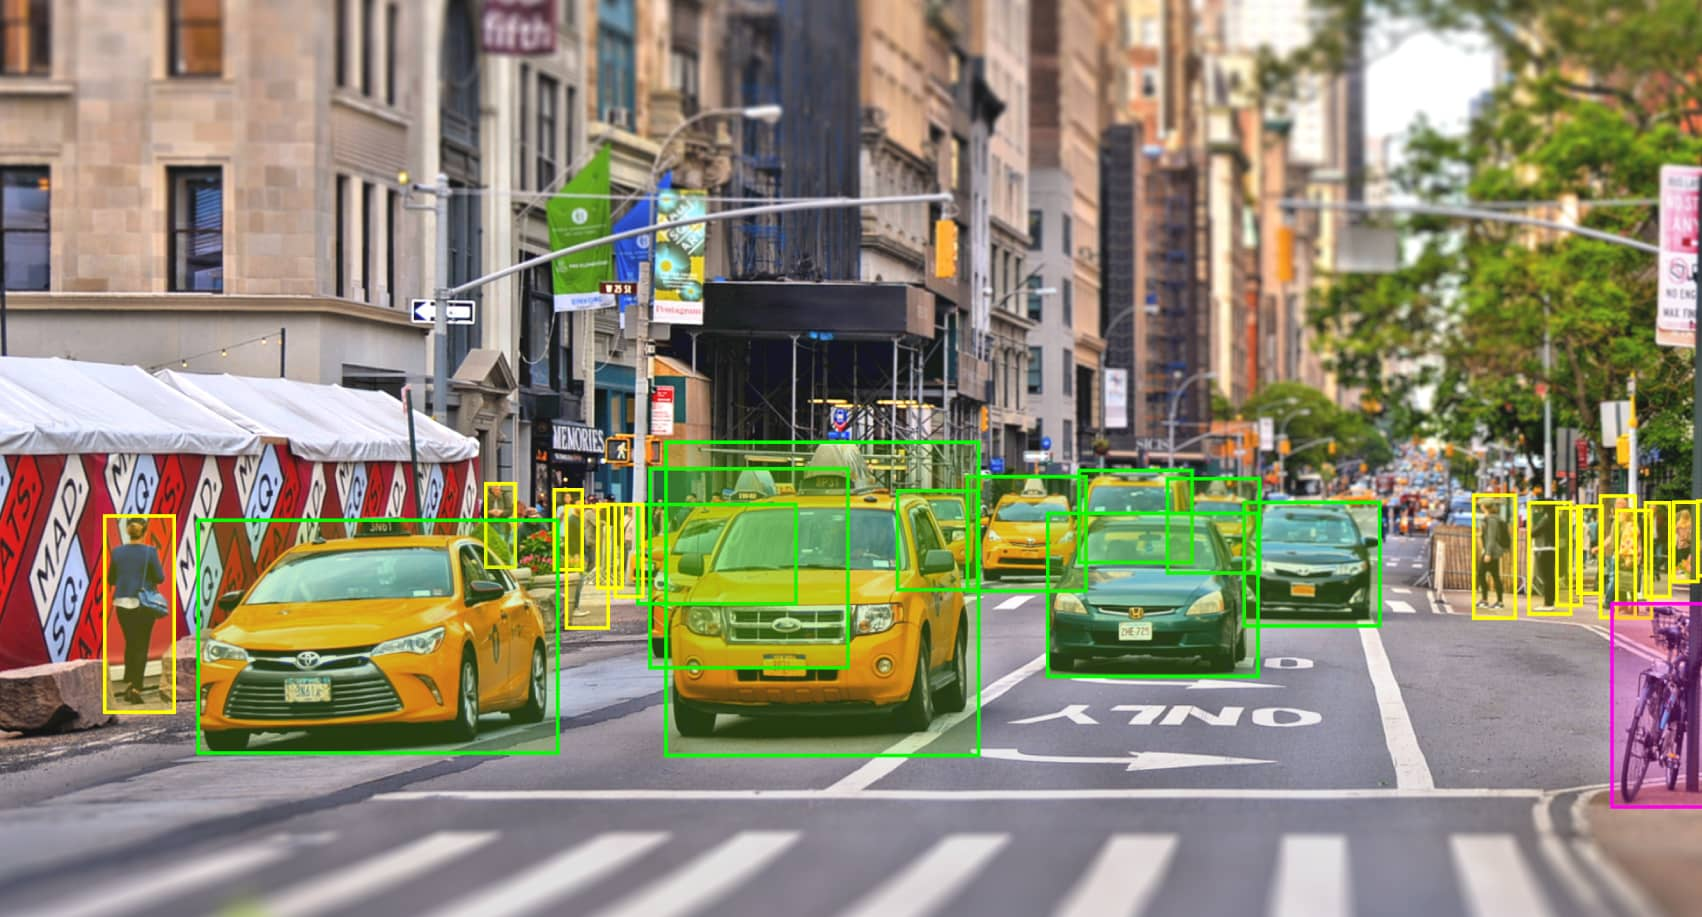
\includegraphics[width=\textwidth]{img/13.jpeg}
				\caption{Illustration d'une annotation de donnée}
			\end{minipage}
		\end{center}
	\end{figure}
	
	\subsubsection{Méthode d'annotation}
	\quad Une méthode d'annotation se réfère à l'approche ou à la technique utilisée pour ajouter des informations ou des métadonnées à une image ou à un ensemble de données d'images. Ces informations peuvent inclure des balises, des étiquettes, des régions d'intérêt, des catégories, des contours, des points clés, etc., en fonction de la tâche spécifique à accomplir.
	
	\textemdash \textbf{ Annotation manuelle : }Les annotateurs humains ajoutent manuellement des balises ou dessinent des régions autour des objets d'intérêt dans les images à l'aide d'outils logiciels spécifiques.
	
	\textemdash \textbf{ Annotation par points clés :}Les annotateurs marquent des points clés ou des points caractéristiques sur des objets dans les images, ce qui est souvent utilisé pour la détection et la reconnaissance d'objets.
	
	\textemdash \textbf{ Annotation par segmentation :}Les annotateurs créent des masques ou des contours autour des objets dans les images pour délimiter les régions d'intérêt, ce qui est couramment utilisé pour la segmentation sémantique.
	
	\textemdash \textbf{ Annotation par classification : }Les annotateurs attribuent des étiquettes ou des catégories à des images entières ou à des parties spécifiques des images en fonction de leur contenu ou de leur classe.
	
	\textemdash \textbf{ Annotation par localisation : }Les annotateurs définissent des boîtes englobantes autour des objets d'intérêt pour indiquer leur emplacement et leur taille dans l'image, ce qui est utilisé pour la détection d'objets. \\
	
	Ces méthodes peuvent être utilisées individuellement ou combinées en fonction des besoins de la tâche d'annotation spécifique.
	
	\subsubsection{Outils d'annotation}
	\quad Les outils d'annotation sont des logiciels ou des plateformes utilisés pour marquer, identifier ou étiqueter des éléments spécifiques dans des données telles que des images, des vidéos ou des documents. Ces annotations comprennent généralement des informations telles que la localisation des objets, les contours, les classes d'objets, etc. L'annotation peut être effectuée manuellement par des opérateurs humains ou automatiquement à l'aide d'algorithmes d'apprentissage automatique. Les données annotées sont essentielles pour entraîner des modèles d'apprentissage automatique supervisés, car elles fournissent des exemples étiquetés sur lesquels le modèle peut apprendre à reconnaître et à interpréter des motifs.
	Voyons ensemble	10 solutions d'annotation automatique:
	
	\begin{itemize}
		\item \textbf{LabelImg : }LabelImg est un outil open-source qui permet d'annoter des images pour la détection d'objets. Il est simple à utiliser et offre la possibilité de définir des boîtes englobantes autour des objets à annoter. Il supporte plusieurs formats d'exportation, tels que XML pour le format Pascal VOC.
		
		Exemple : Un chercheur en vision par ordinateur utilise LabelImg pour annoter des images de voitures afin de créer un ensemble de données pour entraîner un modèle de détection de voitures.
		\item \textbf{LabelMe : }LabelMe est une plateforme en ligne pour l'annotation d'images qui prend en charge la segmentation sémantique, la détection d'objets et d'autres tâches. Il permet également de générer des ensembles de données annotées pour l'apprentissage en profondeur.
		
		Exemple : Une équipe de recherche utilise LabelMe pour annoter des images médicales afin de segmenter les tissus malins dans des scans de tomographie par ordinateur (CT) pour l'analyse de cancer.
		
		\item \textbf{CVAT (Computer Vision Annotation Tool) : }CVAT est une plateforme open-source pour l'annotation d'images et de vidéos. Il offre une interface utilisateur conviviale et prend en charge une variété de tâches d'annotation, y compris la détection d'objets, la classification d'images et la segmentation sémantique.
		
		Exemple : Une entreprise utilise CVAT pour annoter des vidéos de surveillance afin de détecter et suivre automatiquement les mouvements suspects dans les environnements urbains.
		
		\item \textbf{VGG Image Annotator (VIA) : }VIA est un outil open-source d'annotation d'images qui prend en charge divers types d'annotations, y compris les polygones, les boîtes englobantes et les points. Il est léger et facile à utiliser.
		
		Exemple : Un chercheur en écologie utilise VIA pour annoter des images de caméras pièges afin de compter et d'identifier automatiquement les espèces animales dans différentes régions forestières. 
		
		\item \textbf{Labelbox : }Labelbox : Labelbox est une plateforme d'annotation d'images qui offre des fonctionnalités avancées telles que la collaboration en temps réel, la gestion de projet et l'intégration avec des pipelines d'apprentissage automatique.
		
		Exemple : Une start-up utilise Labelbox pour annoter des images satellites afin de cartographier et surveiller les cultures agricoles à grande échelle pour optimiser les rendements.
		
		\item \textbf{COCO Annotator : }COCO Annotator est un outil open-source conçu spécifiquement pour l'annotation d'images dans le format COCO (Common Objects in Context). Il est simple à utiliser et prend en charge la détection d'objets, la segmentation sémantique et la clé d'annotation.
		
		Exemple : Une équipe de recherche utilise COCO Annotator pour annoter des images de rue afin de détecter automatiquement les panneaux de signalisation pour un projet de conduite autonome.
		
		\item \textbf{Amazon SageMaker Ground Truth : }Amazon SageMaker Ground Truth est un service cloud entièrement géré qui facilite l'annotation d'images à grande échelle grâce à l'utilisation de l'apprentissage automatique. Il permet également de valider et de contrôler la qualité des annotations.
		
		Exemple : Une entreprise utilise Amazon SageMaker Ground Truth pour annoter des images médicales afin d'entraîner un modèle d'intelligence artificielle pour la détection automatique des anomalies dans les scans d'IRM.
		
		\item \textbf{Supervisely : }Supervisely est une plateforme d'annotation d'images qui offre des fonctionnalités avancées telles que la segmentation interactive, l'augmentation de données et l'intégration avec des outils d'apprentissage automatique.
		
		Exemple : Une équipe de recherche utilise Supervisely pour annoter des images de drones afin de surveiller et de cartographier les changements environnementaux dans des zones forestières sensibles.
		\item \textbf{OpenLabeling  : }OpenLabeling est un outil open-source d'annotation d'images qui permet de créer des ensembles de données pour l'apprentissage en profondeur. Il offre une flexibilité en termes de formats d'annotation et de types d'annotations pris en charge.
		
		Exemple : Un groupe de passionnés utilise OpenLabeling pour annoter des images de poissons afin de développer un système de reconnaissance automatique des espèces de poissons pour la préservation marine.
	
		\item \textbf{Microsoft VoTT (Visual Object Tagging Tool) :  }    VoTT est un outil open-source développé par Microsoft pour l'annotation d'images et de vidéos. Il est extensible et peut être intégré à des pipelines d'apprentissage automatique.
		
		Exemple : Une entreprise utilise Microsoft VoTT pour annoter des images de produits dans des catalogues en ligne afin d'automatiser le processus de recherche visuelle pour les clients.
	\end{itemize}
	
	\subsection{Une ontologie}
	\quad Une ontologie OWL (Web Ontology Language) est une représentation formelle et structurée de connaissances dans un domaine spécifique. OWL est un langage de représentation des connaissances basé sur le Web, utilisé pour décrire les relations entre les concepts dans un domaine donné. Il est principalement utilisé dans le domaine de la gestion des connaissances, de la sémantique web et de l'intelligence artificielle.
	
	Les ontologies OWL sont construites à l'aide de classes, de propriétés et d'individus. Les classes représentent des ensembles de choses ayant des caractéristiques similaires, les propriétés définissent les relations entre les classes et les individus, et les individus représentent des instances spécifiques de classes.
	
	Les ontologies OWL permettent de formaliser les connaissances de manière à ce qu'elles puissent être interprétées par des machines, facilitant ainsi la recherche, la récupération et l'analyse des informations dans divers domaines d'application. Elles sont largement utilisées dans des domaines tels que la bioinformatique, l'ingénierie des connaissances, la gestion des ressources et bien d'autres encore.
	
	\subsubsection{Rapport entre une ontologie et le web sémantique}
	\begin{itemize}
		\item \textbf{Représentation des connaissances :} Les ontologies sont des structures formelles qui définissent des concepts, des relations et des propriétés dans un domaine particulier. Elles permettent de représenter la connaissance d'un domaine de manière précise et structurée. Le Web sémantique fournit un ensemble de standards et de technologies (comme RDF, OWL et SPARQL) pour représenter et échanger ces ontologies sur le Web, permettant ainsi aux machines de comprendre et d'interpréter les données de manière plus intelligente.
		
		\item \textbf{Interopérabilité des données :} En utilisant des ontologies compatibles avec les standards du Web sémantique, il est possible de créer des données interopérables qui peuvent être partagées et intégrées entre différents systèmes et applications. Cela facilite l'échange de données entre les organisations, les domaines de connaissances et les communautés d'utilisateurs.
		
		\item \textbf{Raisonnement automatique :} Les ontologies permettent de définir des axiomes, des règles et des restrictions sur les données et les concepts d'un domaine. Le Web sémantique fournit des langages et des outils pour réaliser du raisonnement automatique sur ces ontologies, permettant ainsi de déduire de nouvelles connaissances à partir des informations existantes.
		
		\item \textbf{Recherche d'information avancée :} En utilisant les ontologies et les technologies du Web sémantique, il est possible d'améliorer la recherche d'information en permettant aux moteurs de recherche de comprendre le sens des données et des requêtes, plutôt que de se contenter de mots-clés. Cela ouvre la voie à des fonctionnalités de recherche plus avancées et plus précises.
		
		\item \textbf{Applications intelligentes :} La combinaison des ontologies et du Web sémantique permet de développer des applications intelligentes qui exploitent les connaissances formelles pour prendre des décisions, recommander des actions et fournir des services personnalisés. Par exemple, les assistants virtuels, les systèmes d'analyse de données et les systèmes d'aide à la décision peuvent bénéficier de cette approche.
	\end{itemize}
	
	\subsection{Outils}
	\subsubsection{Outils de modélisation ontologique}
	Il existe plusieurs outils permettant de créer une ontologie:
	
	\begin{itemize}
		\item \textbf{TopBraid Composer: } Un outil de modélisation des ontologies et de développement d'applications Web sémantiques, offrant des fonctionnalités avancées pour la création et la 
		\item \textbf{Semantic MediaWiki:} Une extension de MediaWiki qui permet d'ajouter des annotations sémantiques aux pages Wiki, facilitant la création de bases de connaissances sémantiques collaboratives.
		\item \textbf{PoolParty:} Une plateforme de gestion des connaissances sémantiques qui permet la création, l'organisation et la publication d'ontologies et de bases de connaissances sémantiques.
		\item \textbf{RDFLib} Une bibliothèque Python pour travailler avec des données RDF, offrant des fonctionnalités pour la création, la manipulation et le stockage de graphes RDF dans des applications Python.
		\item \textbf{Semantic Web Rule Language (SWRL):}
		\item \textbf{GraphDB:} Une base de données de graphes RDF conçue pour stocker et interroger des données RDF à grande échelle, offrant des fonctionnalités avancées pour la gestion des données sémantiques.
		\item \textbf{Protégé:} Protégé est une plateforme de développement open source qui offre des fonctionnalités de modélisation et de gestion des ontologies. Il est largement utilisé dans le domaine de l'intelligence artificielle et du Web sémantique pour créer, éditer et visualiser des ontologies.
	\end{itemize}


	\section{Chapitre 2 : CONCEPTION}
	\subsection{Introduction}
	\quad Dans cette section, nous nous pencherons sur la conception de notre outil d'annotation, en accordant une attention particulière au développement de l'ontologie. L'ontologie revêt une importance fondamentale au sein de notre système, car elle fournit une structure conceptuelle qui nous permet de représenter et de modéliser les connaissances spécifiques à notre domaine d'étude. Nous détaillerons le processus de création de l'ontologie en décrivant les différentes classes, propriétés et relations utilisées pour dépeindre les entités et les concepts clés. En outre, nous présenterons un processus d'annotation qui tire parti de l'ontologie pour guider et faciliter l'annotation des données en leur attribuant une signification sémantique.
	
	\subsection{Annotation}
	Le processus d'annotation est segmenté en plusieurs phases :
	
	\textemdash \textbf{ Acquisition d'images de maniocs }: Cette étape implique la collecte d'images illustrant les différentes affections et la santé des plants de manioc.
	
	\textemdash \textbf{ Prétraitement des images : }Avant d'entamer l'extraction des caractéristiques, il est généralement requis de prétraiter les images afin d'en améliorer la qualité. Cette phase comprend plusieurs opérations visant à optimiser les données visuelles.
	
	\textemdash \textbf{ Extraction des caractéristiques :}À ce stade, des algorithmes spécialisés sont employés pour extraire des informations pertinentes des images, en se fondant sur les divers symptômes associés aux maladies affectant le manioc.
	
	\textemdash \textbf{ Annotation sémantique : }Cette étape implique l'utilisation d'une ontologie pour annoter les caractéristiques extraites. Elle vise à enrichir le processus de détection des maladies et à appliquer des inférences basées sur l'ontologie pour accroître la précision de la détection.
	
	\begin{figure}[htbp]
		\begin{center}
			\begin{minipage}[b]{0.7\textwidth}
				\centering
				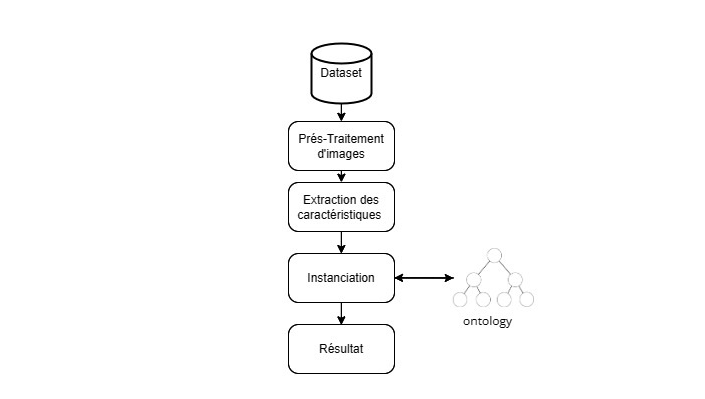
\includegraphics[width=\textwidth]{img/14.png}
				\caption{Illustration d'un processus annotation}
			\end{minipage}
		\end{center}
	\end{figure}
	
	\subsection{Mise en place de l'ontologie}
	Dans le cadre de l'annotation sémantique, la mise en place d'une ontologie vise principalement à fournir une structure conceptuelle formelle pour représenter et organiser les connaissances spécifiques à un domaine donné. Voici quelques objectifs clés de l'utilisation d'une ontologie dans ce contexte :
	
	\begin{description}
		\item[Structurer les connaissances : ]L'ontologie permet de définir des concepts, des classes, des propriétés et des relations qui représentent les entités et les concepts clés du domaine. Cela offre une structure organisée pour les données annotées, facilitant ainsi la recherche, l'analyse et la compréhension des informations.
		
		\item[Normalisation et standardisation : ]En établissant des termes normalisés et des relations standardisées, une ontologie favorise la cohérence et l'interopérabilité des données annotées. Cela permet aux différents utilisateurs et systèmes de partager et d'échanger efficacement des informations.
		
		\item[Enrichir la sémantique :] L'ontologie attribue une signification explicite aux annotations en définissant des termes et des relations avec précision. Cela permet une compréhension plus approfondie des données et des processus, en offrant un contexte sémantique qui facilite l'interprétation et l'analyse.
		
		\item[Guider le processus d'annotation : ]L'ontologie fournit un cadre de référence pour guider le processus d'annotation en spécifiant les concepts à annoter, les relations à établir et les contraintes à respecter. Cela contribue à assurer la cohérence et la qualité des annotations réalisées par les annotateurs.
		
		\item[Faciliter l'inférence et l'analyse :]En utilisant une ontologie, il est possible d'effectuer des raisonnements basés sur les relations définies entre les concepts. Cela permet d'inférer de nouvelles informations à partir des données annotées, d'identifier des corrélations et des tendances, et d'effectuer des analyses avancées sur les données.
		
	
	\end{description}
	
		En résumé, l'objectif principal de la mise en place d'une ontologie dans le cadre de l'annotation sémantique est de fournir un cadre formel et structuré pour représenter, organiser et interpréter les connaissances, ce qui contribue à améliorer la qualité, la cohérence et la valeur des données annotées. \\
		
		Nous nous baserons sur [31] pour la construction de notre ontologie axé sur les images. Elle est repartie en 8 etapes qui sont : 
		
		
		\begin{enumerate}
			\item  \textbf{ Définition du domaine et des objectifs de l’ontologie :}Nous visons à développer une ontologie dédiée à l'annotation sémantique automatique des images pour la détection des symptômes des maladies du manioc. L'objectif principal est de fournir une structure conceptuelle précise et spécialisée pour faciliter cette annotation automatique, améliorant ainsi la précision et l'efficacité du processus de détection des maladies du manioc.
			
			\item  \textbf{ Exploration et analyse des sources pertinentes :}Nous collectons et analysons les informations disponibles pour comprendre le domaine et ses spécificités.
			
			\item  \textbf{ Identification des concepts essentiels et de leurs relations :}Nous identifions les principaux concepts et établissons leurs relations pour structurer notre ontologie de manière cohérente.
			
			\item  \textbf{ Hiérarchisation des concepts et création de classes : } Nous organisons les concepts en hiérarchies pour mieux représenter les relations entre eux et créons des classes pour chaque catégorie identifiée.
			
			\item  \textbf{ Définition des propriétés pour chaque classe :} Nous définissons les caractéristiques et les attributs associés à chaque classe pour enrichir la représentation des concepts dans notre ontologie.
			
			\item  \textbf{ Création d'instances pour chaque classe :}Nous créons des exemples concrets ou des instances pour chaque classe afin d'illustrer leur utilisation et leur fonctionnement dans le domaine.
			
			\item  \textbf{ Validation de l'ontologie avec des exemples concrets : } Nous validons notre ontologie en l'appliquant à des cas réels pour vérifier sa pertinence et son efficacité dans la détection des symptômes des maladies du manioc.
			
			\item  \textbf{ Révision et mise à jour de l'ontologie si nécessaire :}Nous révisons et mettons à jour l'ontologie en fonction des retours d'expérience et des évolutions du domaine pour garantir sa pertinence et sa fiabilité au fil du temps.
			
			
		\end{enumerate}
		
		
		\subsubsection{Collecte d´information (Le Dataset)}
		Pour obtenir des informations sur les maladies du manioc, nous avons exploité diverses sources pour recueillir des données précises et fiables. Nous avons examiné des articles scientifiques spécialisés dans le domaine de l'agriculture ainsi que des rapports de recherche [*], [*], [*]. Ces ressources nous ont fourni des détails sur les différentes maladies que trouvons sur chez le manioc, ainsi que sur les symptômes, les causes et les traitements associés à chacune d'entre elles.
		
		\quad Dans cette étude, nous examinons comment utiliser des techniques spéciales pour comprendre et détecter les maladies du manioc à partir d'images des feuilles, des tiges ou des racines infectées.
		
		\quad La culture du manioc est confrontée à diverses menaces, notamment des maladies qui peuvent avoir un impact significatif sur la production et la qualité des récoltes. Parmi les maladies les plus préoccupantes\cite{msikita_lutte_nodate}, on trouve : \\ \\
		\textemdash \textbf{  Maladie de la Mosaïque du Manioc, } \\
		\textemdash \textbf{ Maladie de la Tache Brune du Manioc, } \\
		\textemdash \textbf{ Flétrissement Bactérien du Manioc, } \\
		\textemdash \textbf{ Acarien Vert du Manioc, } \\
		\textemdash \textbf{  Pourriture des Racines du Manioc, } \\
		\textemdash \textbf{ Anthracnose du ManiocAnthracnose du Manioc, } \\
		\textemdash \textbf{ Flétrissement Bactérien du Manioc, } \\
		\textemdash \textbf{ Maladie Rose du Manioc, } \\
		\textemdash \textbf{ Nanisme du Manioc } \\
		\textemdash \textbf{ Tache Foliaire du Manioc } \\	
		\textemdash \textbf{ Nématode à Nœuds Radiculaires du Manioc } \\	
		\textemdash \textbf{ Moucheron Blanc du Manioc } \\	
		\textemdash \textbf{ Etc } \\	
		
		Dans cette étude, nous nous concentrerons sur l'analyse sémantique des images pour détecter et comprendre ces maladies spécifiques du manioc. En s'inspirant des images données par notre enseignant, nous mettrons donc l'accent sur : \\ \\
		\textemdash \textbf{ Brûlure bactérienne (Bacterial Blight (CBB)), } \\
		\textemdash \textbf{ Maladie des stries brunes (Brown Streak Disease (CBSD)), } \\
		\textemdash \textbf{ Marbrure verte (Green Mottle (CGM)), } \\
		\textemdash \textbf{ Maladie de la mosaïque (Mosaic Disease (CMD)) } \\
		
		Grâce aux images de maladies fournies par notre enseignant, soit plus de 4 000 images,
		ainsi qu'à nos recherches sur [*], nous avons réussi à rassembler plus de 20 000 images.
		La plus part etant deorganiser, nous les oavions regorganiser en les en differents classes(dossiers) grace a python a travers ce code : \\
		
		\textbf{Avant la classification des images}
		\begin{figure}[htbp]
			\begin{center}
				\begin{minipage}[b]{0.7\textwidth}
					\centering
					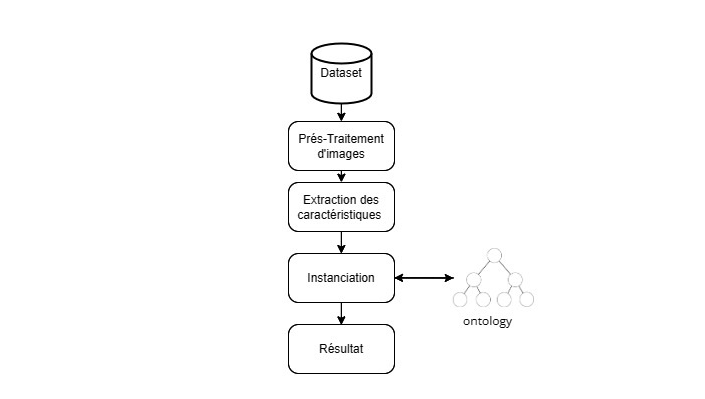
\includegraphics[width=\textwidth]{img/14.png}
					\caption{Avant la classification}
				\end{minipage}
			\end{center}
		\end{figure}
		
		\textbf{ Implementation du code de classification des images}
		\begin{figure}[htbp]
			\begin{center}
				\begin{minipage}[b]{0.7\textwidth}
					\centering
					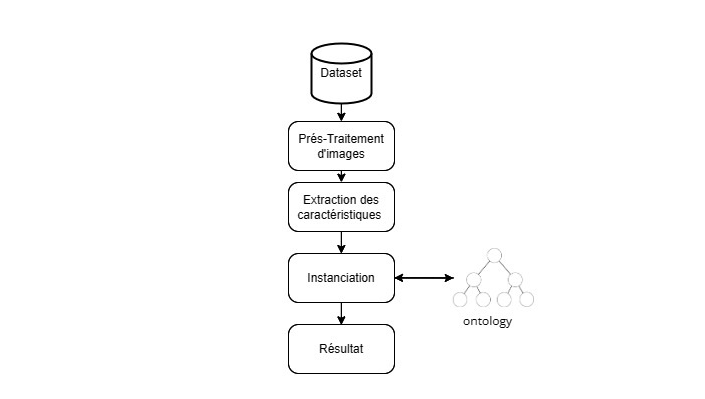
\includegraphics[width=\textwidth]{img/14.png}
					\caption{Le code de classification}
				\end{minipage}
			\end{center}
		\end{figure}
		
		\textbf{ Après la classification des images }
		\begin{figure}[htbp]
			\begin{center}
				\begin{minipage}[b]{0.7\textwidth}
					\centering
					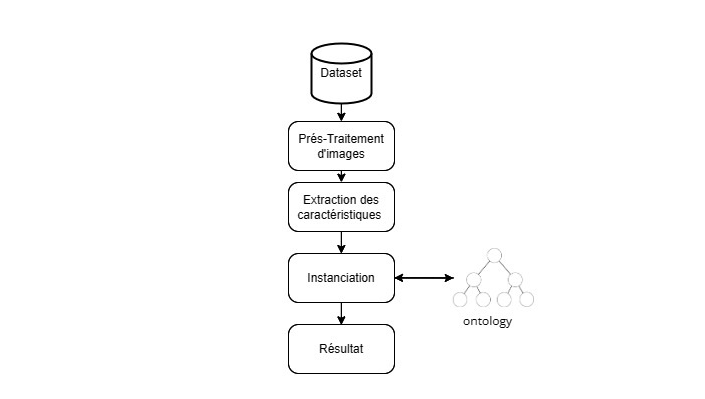
\includegraphics[width=\textwidth]{img/14.png}
					\caption{Après la classification}
				\end{minipage}
			\end{center}
		\end{figure}
		
		\paragraph{Brûlure bactérienne (Bacterial Blight (CBB))}
		\begin{itemize}
			\item \textbf{Images: }
			\begin{figure}[htbp]
				\centering
				\begin{subfigure}[b]{0.3\textwidth}
					\centering
					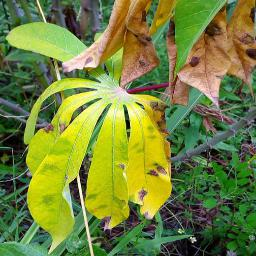
\includegraphics[width=\textwidth]{img/1.jpg}
					\caption{Bactérienne 1}
				\end{subfigure}
				\hfill
				\begin{subfigure}[b]{0.3\textwidth}
					\centering
					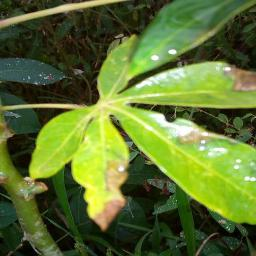
\includegraphics[width=\textwidth]{img/2.jpg}
					\caption{Bactérienne 2}
				\end{subfigure}
				\hfill
				\begin{subfigure}[b]{0.3\textwidth}
					\centering
					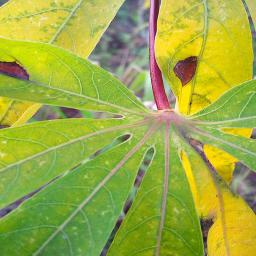
\includegraphics[width=\textwidth]{img/3.jpg}
					\caption{Bactérienne 3}
				\end{subfigure}
				\caption{Images de la brûlure bactérienne}
			\end{figure}
			\item \textbf{Définition: } La brûlure bactérienne est caractérisée par l'apparition de taches nécrotiques, humides et brunes sur les feuilles du manioc. 
			\item \textbf{Cause: } La brûlure bactérienne est une maladie causée par des bactéries qui affectent les plantes, provoquant l'apparition de taches nécrosées sur les feuilles, entraînant souvent le flétrissement, la mort des feuilles et une diminution de la vigueur de la plante.
			\item \textbf{Symptôme: } La bactériose du manioc se présente d'abord sous forme de petites taches humides sur les feuilles, qui deviennent ensuite de plus en plus grandes et brunissent le limbe. Les feuilles touchées finissent par flétrir, mourir et tomber. Ce problème est plus grave pendant la saison des pluies et affecte principalement les jeunes plants.
			\item \textbf{Traitement: } Le traitement de la bactériose du manioc peut impliquer l'utilisation de cultivars résistants, des pratiques culturales appropriées et, parfois, l'application de produits chimiques comme des pesticides.
		\end{itemize}
		
		\paragraph{Maladie des stries brunes (Brown Streak Disease (CBSD))}
		\begin{itemize}
			\item \textbf{Images: }
			\begin{figure}[htbp]
				\centering
				\begin{subfigure}[b]{0.3\textwidth}
					\centering
					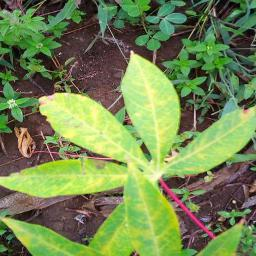
\includegraphics[width=\textwidth]{img/4.jpg}
					\caption{Stries brunes 4}
				\end{subfigure}
				\hfill
				\begin{subfigure}[b]{0.3\textwidth}
					\centering
					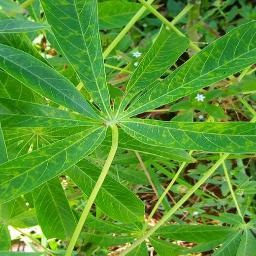
\includegraphics[width=\textwidth]{img/5.jpg}
					\caption{Stries brunes 5}
				\end{subfigure}
				\hfill
				\begin{subfigure}[b]{0.3\textwidth}
					\centering
					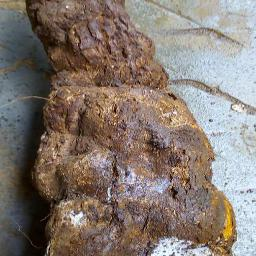
\includegraphics[width=\textwidth]{img/6.jpg}
					\caption{Stries brunes 6}
				\end{subfigure}
				\caption{Images de la maladie des stries brunes}
			\end{figure}
			
			\item \textbf{Définition: } Elle se caractérise par l'apparition de stries brunes sur les racines et les tubercules du manioc infecté, ce qui entraîne une réduction de la qualité et de la quantité des récoltes.
			\item \textbf{Cause: } La Maladie des stries brunes, ou Brown Streak Disease (CBSD), est principalement causée par deux virus du groupe des potyvirus : le virus de la maladie des stries brunes de l'est (BSeMV) et le virus de la maladie des stries brunes de l'ouest (BScMV).
			\item \textbf{Symptôme: } La maladie des stries brunes se manifeste par des symptômes observables sur les feuilles, les tiges et les tubercules du manioc. Sur les feuilles, elle se caractérise par l'apparition de taches jaune-vert, plus prononcées sur les feuilles développées. Contrairement à la mosaïque, les feuilles touchées ne se déforment pas. Sur les tiges, des stries brun foncé ainsi que des lésions nécrotiques peuvent apparaître, principalement sur la partie supérieure verte. Les tubercules peuvent également être déformés, présenter des craquelures et une décoloration.
			\item \textbf{Traitement: } Le traitement de la maladie des stries brunes du manioc peut être difficile car il n'existe pas de méthode curative complètement efficace une fois que la plante est infectée. Cependant, plusieurs approches de gestion peuvent être utilisées pour réduire la propagation de la maladie et limiter ses effets sur les cultures :
			
			\textemdash  Utilisation de cultivars résistants : Sélectionner et cultiver des variétés de manioc qui sont résistantes ou tolérantes à la maladie peut aider à réduire la propagation de la maladie dans les cultures.
			
			\textemdash  Contrôle des vecteurs : La gestion des insectes vecteurs, tels que les pucerons, peut réduire la transmission des virus responsables de la maladie.
			
			\textemdash  Pratiques culturales appropriées : Adopter des pratiques culturales telles que la rotation des cultures, la gestion de l'irrigation et la suppression des plantes infectées peut contribuer à réduire la propagation de la maladie dans les champs.
			
			\textemdash  Utilisation de matériel de plantation sain : Utiliser des boutures de manioc exemptes de maladie pour la plantation peut aider à réduire la propagation de la maladie lors de la multiplication des cultures.
		\end{itemize}
		
		
		
		\paragraph{Marbrure verte (Green Mottle (CGM))}
		\begin{itemize}
			\item \textbf{Images: }
			\begin{figure}[htbp]
				\centering
				\begin{subfigure}[b]{0.3\textwidth}
					\centering
					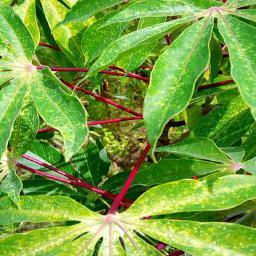
\includegraphics[width=\textwidth]{img/7.jpg}
					\caption{Marbrure verte 7}
				\end{subfigure}
				\hfill
				\begin{subfigure}[b]{0.3\textwidth}
					\centering
					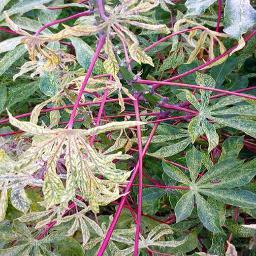
\includegraphics[width=\textwidth]{img/8.jpg}
					\caption{Marbrure verte 8}
				\end{subfigure}
				\hfill
				\begin{subfigure}[b]{0.3\textwidth}
					\centering
					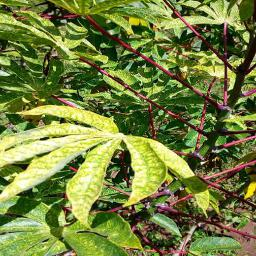
\includegraphics[width=\textwidth]{img/9.jpg}
					\caption{Marbrure verte 9}
				\end{subfigure}
				\caption{Images de la marbrure verte}
			\end{figure}
			
			\item \textbf{Définition: } La Marbrure verte (Green Mottle ou CGM) du manioc se caractérise par l'apparition de marbrures vert clair ou jaune-vert sur les feuilles infectées. Ces marbrures peuvent être irrégulières et s'étendre sur toute la surface des feuilles. Les symptômes sont généralement plus visibles sur la face supérieure des feuilles et peuvent varier en intensité selon le degré d'infection et les conditions environnementales.
			\item \textbf{Cause: } La Marbrure verte (Green Mottle ou CGM) du manioc est principalement causée par une infection virale. Le virus responsable de cette maladie est transmis par des insectes vecteurs, tels que les aleurodes (mouches blanches), qui se nourrissent de la sève des plantes infectées et propagent ainsi le virus à d'autres plantes saines.
			\item \textbf{Symptôme: } Les symptômes de la Marbrure verte (Green Mottle ou CGM) sur les feuilles du manioc se manifestent généralement par l'apparition de marbrures vert clair ou jaune-vert. Ces marbrures peuvent être irrégulières et se propager sur toute la surface des feuilles. Les feuilles affectées peuvent également présenter des déformations et un rabougrissement. Les symptômes peuvent varier en fonction de la gravité de l'infection et des conditions environnementales.
			\item \textbf{Traitement: } Le traitement de la Marbrure verte du manioc (Green Mottle ou CGM) est principalement axé sur la gestion des populations d'insectes vecteurs responsables de la transmission du virus. Voici quelques mesures de gestion qui peuvent être adoptées :
			
			\textemdash  Contrôle des insectes vecteurs : Utilisation de méthodes de lutte intégrée telles que l'utilisation de pièges, de filets anti-insectes et de produits phytosanitaires pour réduire les populations d'insectes vecteurs, comme les aleurodes.
			
			\textemdash  Cultivars résistants : Sélection et plantation de variétés de manioc résistantes ou tolérantes à la maladie, si disponibles.
			
			\textemdash  Rotation des cultures : Pratique consistant à alterner les cultures de manioc avec d'autres cultures non sensibles à la maladie pour réduire la pression des vecteurs et la propagation du virus.
			
			\textemdash  Élimination des plantes infectées : Enlever et détruire les plantes infectées dès l'apparition des symptômes pour réduire la source de l'inoculum viral dans les champs.
		\end{itemize}
		
		
		\paragraph{Maladie de la mosaïque (Mosaic Disease (CMD))}
		\begin{itemize}
			\item \textbf{Images: }
			\begin{figure}[htbp]
				\centering
				\begin{subfigure}[b]{0.3\textwidth}
					\centering
					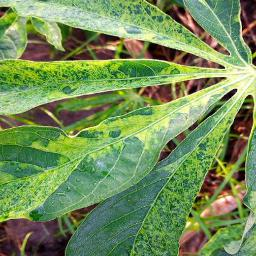
\includegraphics[width=\textwidth]{img/10.jpg}
					\caption{Mosaïque 10}
				\end{subfigure}
				\hfill
				\begin{subfigure}[b]{0.3\textwidth}
					\centering
					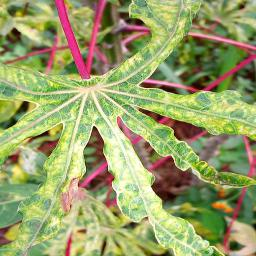
\includegraphics[width=\textwidth]{img/11.jpg}
					\caption{Mosaïque 11}
				\end{subfigure}
				\hfill
				\begin{subfigure}[b]{0.3\textwidth}
					\centering
					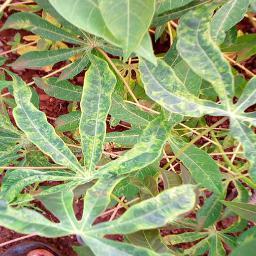
\includegraphics[width=\textwidth]{img/12.jpg}
					\caption{Mosaïque 12}
				\end{subfigure}
				\caption{Images de la maladie de la mosaïque}
			\end{figure}
			
			\item \textbf{Définition: } La Maladie de la mosaïque du manioc se caractérise par l'apparition de motifs de mosaïque sur les feuilles des plants infectés. Ces motifs se présentent sous forme de zones de couleur verte et jaune irrégulières et distinctes.
			\item \textbf{Cause: } La mosaïque du manioc est causée par un virus
			qui s’introduit dans les feuilles et les tiges du
			manioc.
			\item \textbf{Symptôme: } La Maladie de la mosaïque du manioc est principalement causée par des virus, tels que le virus de la mosaïque du manioc (Cassava Mosaic Virus, CMV) et d'autres virus apparentés du groupe des begomovirus. Ces virus sont transmis par des pucerons vecteurs lorsqu'ils se nourrissent de la sève des plantes infectées.
			\item \textbf{Traitement: } Il n'existe pas de traitement curatif pour la Maladie de la mosaïque du manioc une fois que les plantes sont infectées par le virus. Cependant, plusieurs mesures peuvent être prises pour réduire les risques d'infection et limiter les dommages causés par la maladie :
			
			\textemdash  Utilisation de cultivars résistants : Planter des variétés de manioc qui sont génétiquement résistantes ou tolérantes à la Maladie de la mosaïque du manioc peut aider à réduire la propagation de la maladie dans les cultures.
			
			\textemdash  Contrôle des vecteurs : Mettre en place des mesures de contrôle des pucerons vecteurs, tels que l'utilisation de pièges, de filets anti-insectes et de produits phytosanitaires, peut aider à réduire la transmission du virus.
			
			\textemdash  Pratiques culturales appropriées : Adopter des pratiques culturales telles que la rotation des cultures, la gestion de l'irrigation et l'élimination des mauvaises herbes peut contribuer à réduire la pression des vecteurs et la propagation du virus.
		\end{itemize}
		
		Quand nous examinons une image de manioc affecté par une maladie, nous remarquons que cette image présente les aspects suivants : la forme, la teinte, la texture et des perforations.
		Explorons de manière approfondie ces caractéristiques :
		
		\begin{itemize}
			\item  \textbf{ Couleur (Color) :} Il s'agit de la teinte ou de la couleur dominante présente dans l'image. La couleur peut fournir des informations sur l'état de santé de la plante, par exemple des taches jaunes ou brunes indiquant une maladie.
			
			\item  \textbf{ Forme (Shape) :} Cette caractéristique fait référence à la silhouette ou à la structure globale des éléments dans l'image. Par exemple, la forme des feuilles ou des lésions sur les feuilles peut être analysée pour détecter des signes de maladies.
			
			\item  \textbf{ Texture (Texture) :}La texture se réfère aux variations dans la structure de surface de l'image. Cela peut inclure des motifs ou des arrangements de pixels qui indiquent des caractéristiques spécifiques, comme la rugosité ou la douceur des feuilles.
			
			\item  \textbf{ Trous (Holes) :}Cette caractéristique pourrait faire référence à la présence de trous ou de lacunes dans les feuilles ou d'autres parties de la plante, ce qui pourrait indiquer des dommages causés par des insectes ou des maladies.
		\end{itemize}
		
		
	\subsubsection{Conceptualisation (Prés-traitement des images)}
	Dans cette partie, nous explorerons les éléments fondamentaux de la création de l'ontologie, ce qui inclut la clarification des concepts, la détermination des attributs, et la configuration des relations.
	\textbf{ Clarification des concepts : } cette phase implique d'établir une liste des concepts identifiés durant la collecte d'informations.
	
	\begin{table}[htbp]
		\centering
		\begin{tabular}{|p{0.45\textwidth}|p{0.45\textwidth}|} % Définit deux colonnes de largeur 45% de la largeur de la page
			\hline
			\textbf{Image} & \textbf{Symptom} \\
			\hline
			Représente une représentation visuelle ou graphique d’un plant de blé ou d’une partie de celui-ci. Il capture les propriétés d'une image. & Représente les manifestations cliniques ou visuelles observées sur les grains de blé qui sont associées à des maladies spécifiques. \\
			\hline
		\end{tabular}
		\caption{Liste des concepts identifiés}

	\end{table}
	
	
	
	\textbf{ Établir les propriétés : }Cette phase implique la définition des propriétés associées à chaque concept, décrivant ainsi leurs caractéristiques spécifiques. \\
	
	\textbf{ Établir les relations : }Cette étape consiste à établir des liens logiques entre les concepts et les propriétés pour refléter les interrelations entre les différentes entités.
	
	\begin{table}[htbp]
		\centering
		\begin{tabular}{|p{5cm}|p{5cm}|p{5cm}|} % Définit trois colonnes centrées
			\hline
			\textbf{Propriété} & \textbf{Domain} & \textbf{Range} \\
			\hline
			hasCouleur & Image & String \\
			\hline
			hasTexture & Image & String \\
			\hline
			hasForme & Image & String \\
			\hline
			hasHols & Image & Boolean \\
			\hline
		\end{tabular}
		\caption{Liste des propriété}

	\end{table}
	
	
	\begin{table}[htbp]
		\centering
		\begin{tabular}{|p{5cm}|p{5cm}|p{5cm}|} % Définit trois colonnes de largeur 4cm
			\hline
			\textbf{Relation} & \textbf{Domain} & \textbf{Range} \\
			\hline
			hasImage & Dataset & Image \\
			\hline
		\end{tabular}
		\caption{Liste des relations}

	\end{table}
	

	\newpage
	\section{Bibliographies}
	
	\bibliographystyle{plain} % Style de la bibliographie
	\bibliography{c} % Nom du fichier .bib (sans l'extension)
	%\bibliographystyle{smfplain}
	
\end{document}
